\mbox{$\displaystyle -\,$\,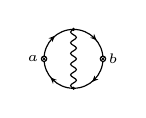
\begin{tikzpicture}[x=0.340cm, y=0.340cm, line width=0.420pt, baseline={([yshift=-0.6ex]0,0)}]
  \draw (0.000,-1.100) arc[start angle=270.000, end angle=180.000, radius=1.100];
  \fill (-0.862,-0.693) -- (-0.766,-0.934) -- (-0.748,-0.807) -- (-0.621,-0.790) -- cycle;
  \draw (0.000,1.100) arc[start angle=90.000, end angle=0.000, radius=1.100];
  \fill (0.862,0.693) -- (0.766,0.934) -- (0.748,0.807) -- (0.621,0.790) -- cycle;
  \draw (1.100,0.000) arc[start angle=0.000, end angle=-90.000, radius=1.100];
  \fill (0.693,-0.862) -- (0.934,-0.766) -- (0.807,-0.748) -- (0.790,-0.621) -- cycle;
  \draw (-1.100,0.000) arc[start angle=180.000, end angle=90.000, radius=1.100];
  \fill (-0.693,0.862) -- (-0.934,0.766) -- (-0.807,0.748) -- (-0.790,0.621) -- cycle;
  \draw plot[smooth, tension=0.7] coordinates {(0.000,-1.100) (-0.076,-1.050) (-0.108,-1.000) (-0.076,-0.950) (0.000,-0.900) (0.076,-0.850) (0.108,-0.800) (0.076,-0.750) (0.000,-0.700) (-0.076,-0.650) (-0.108,-0.600) (-0.076,-0.550) (0.000,-0.500) (0.076,-0.450) (0.108,-0.400) (0.076,-0.350) (0.000,-0.300) (-0.076,-0.250) (-0.108,-0.200) (-0.076,-0.150) (0.000,-0.100) (0.076,-0.050) (0.108,0.000) (0.076,0.050) (0.000,0.100) (-0.076,0.150) (-0.108,0.200) (-0.076,0.250) (0.000,0.300) (0.076,0.350) (0.108,0.400) (0.076,0.450) (0.000,0.500) (-0.076,0.550) (-0.108,0.600) (-0.076,0.650) (0.000,0.700) (0.076,0.750) (0.108,0.800) (0.076,0.850) (0.000,0.900) (-0.076,0.950) (-0.108,1.000) (-0.076,1.050) (0.000,1.100)};
  \draw[fill=white] (-1.100,0.000) circle (0.100);
  \draw[line width=0.298pt] (-1.030,0.070) -- (-1.170,-0.070) (-1.030,-0.070) -- (-1.170,0.070);
  \draw[fill=white] (1.100,0.000) circle (0.100);
  \draw[line width=0.298pt] (1.170,0.070) -- (1.030,-0.070) (1.170,-0.070) -- (1.030,0.070);
  \fill (0.000,-1.100) circle (0.064);
  \fill (0.000,1.100) circle (0.064);
  \node[font=\tiny, inner sep=0pt, anchor=0] at (-1.290,0.000) {$a$};
  \node[font=\tiny, inner sep=0pt, anchor=180] at (1.290,0.000) {$b$};
\end{tikzpicture}}
\diagramgap
\mbox{$\displaystyle +\,$\,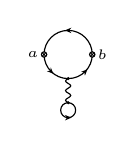
\begin{tikzpicture}[x=0.340cm, y=0.340cm, line width=0.420pt, baseline={([yshift=-0.6ex]0,0)}]
  \draw (0.900,0.000) arc[start angle=0.000, end angle=180.000, radius=0.900];
  \fill (-0.119,0.900) -- (0.119,0.798) -- (0.042,0.900) -- (0.119,1.002) -- cycle;
  \draw (0.000,-0.900) arc[start angle=270.000, end angle=360.000, radius=0.900];
  \fill (0.721,-0.552) -- (0.480,-0.649) -- (0.607,-0.666) -- (0.624,-0.793) -- cycle;
  \draw (-0.900,0.000) arc[start angle=180.000, end angle=270.000, radius=0.900];
  \fill (-0.552,-0.721) -- (-0.649,-0.480) -- (-0.666,-0.607) -- (-0.793,-0.624) -- cycle;
  \draw plot[smooth, tension=0.7] coordinates {(0.000,-1.800) (-0.069,-1.755) (-0.097,-1.710) (-0.069,-1.665) (0.000,-1.620) (0.069,-1.575) (0.097,-1.530) (0.069,-1.485) (0.000,-1.440) (-0.069,-1.395) (-0.097,-1.350) (-0.069,-1.305) (0.000,-1.260) (0.069,-1.215) (0.097,-1.170) (0.069,-1.125) (0.000,-1.080) (-0.069,-1.035) (-0.097,-0.990) (-0.069,-0.945) (0.000,-0.900)};
  \draw (0.000,-1.800) arc[start angle=90.000, end angle=450.000, radius=0.280];
  \fill (0.119,-2.360) -- (-0.119,-2.258) -- (-0.042,-2.360) -- (-0.119,-2.462) -- cycle;
  \draw[fill=white] (-0.900,0.000) circle (0.100);
  \draw[line width=0.298pt] (-0.830,0.070) -- (-0.970,-0.070) (-0.830,-0.070) -- (-0.970,0.070);
  \draw[fill=white] (0.900,0.000) circle (0.100);
  \draw[line width=0.298pt] (0.970,0.070) -- (0.830,-0.070) (0.970,-0.070) -- (0.830,0.070);
  \fill (0.000,-1.800) circle (0.064);
  \fill (0.000,-0.900) circle (0.064);
  \node[font=\tiny, inner sep=0pt, anchor=0] at (-1.090,0.001) {$a$};
  \node[font=\tiny, inner sep=0pt, anchor=180] at (1.090,0.001) {$b$};
\end{tikzpicture}}
\diagramgap
\mbox{$\displaystyle -\,$\,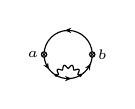
\begin{tikzpicture}[x=0.340cm, y=0.340cm, line width=0.420pt, baseline={([yshift=-0.6ex]0,0)}]
  \draw (0.900,0.000) arc[start angle=0.000, end angle=180.000, radius=0.900];
  \fill (-0.119,0.900) -- (0.119,0.798) -- (0.042,0.900) -- (0.119,1.002) -- cycle;
  \draw (0.450,-0.779) arc[start angle=300.000, end angle=360.000, radius=0.900];
  \fill (0.839,-0.347) -- (0.631,-0.502) -- (0.759,-0.486) -- (0.808,-0.604) -- cycle;
  \draw (-0.450,-0.779) arc[start angle=240.000, end angle=300.000, radius=0.900];
  \fill (0.119,-0.900) -- (-0.119,-0.798) -- (-0.042,-0.900) -- (-0.119,-1.002) -- cycle;
  \draw plot[smooth, tension=0.7] coordinates {(0.450,-0.779) (0.394,-0.766) (0.363,-0.748) (0.368,-0.713) (0.393,-0.660) (0.412,-0.604) (0.404,-0.562) (0.363,-0.549) (0.305,-0.562) (0.250,-0.580) (0.215,-0.581) (0.200,-0.549) (0.193,-0.491) (0.179,-0.433) (0.150,-0.402) (0.109,-0.413) (0.066,-0.455) (0.030,-0.500) (0.000,-0.519) (-0.030,-0.500) (-0.066,-0.455) (-0.109,-0.413) (-0.150,-0.402) (-0.179,-0.433) (-0.193,-0.491) (-0.200,-0.549) (-0.215,-0.581) (-0.250,-0.580) (-0.305,-0.562) (-0.363,-0.549) (-0.404,-0.562) (-0.412,-0.604) (-0.393,-0.660) (-0.368,-0.713) (-0.363,-0.748) (-0.394,-0.766) (-0.450,-0.779)};
  \draw (-0.900,0.000) arc[start angle=180.000, end angle=240.000, radius=0.900];
  \fill (-0.720,-0.553) -- (-0.751,-0.296) -- (-0.800,-0.414) -- (-0.927,-0.398) -- cycle;
  \draw[fill=white] (-0.900,0.000) circle (0.100);
  \draw[line width=0.298pt] (-0.830,0.070) -- (-0.970,-0.070) (-0.830,-0.070) -- (-0.970,0.070);
  \draw[fill=white] (0.900,0.000) circle (0.100);
  \draw[line width=0.298pt] (0.970,0.070) -- (0.830,-0.070) (0.970,-0.070) -- (0.830,0.070);
  \fill (0.450,-0.779) circle (0.064);
  \fill (-0.450,-0.779) circle (0.064);
  \node[font=\tiny, inner sep=0pt, anchor=359] at (-1.090,0.002) {$a$};
  \node[font=\tiny, inner sep=0pt, anchor=181] at (1.090,0.002) {$b$};
\end{tikzpicture}}
\diagramgap
\mbox{$\displaystyle +\,$\,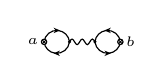
\begin{tikzpicture}[x=0.340cm, y=0.340cm, line width=0.420pt, baseline={([yshift=-0.6ex]0,0)}]
  \draw (-0.475,0.000) arc[start angle=353.974, end angle=186.026, radius=0.478];
  \fill (-1.069,-0.427) -- (-0.831,-0.530) -- (-0.908,-0.427) -- (-0.831,-0.325) -- cycle;
  \draw (-1.425,0.000) arc[start angle=173.974, end angle=6.026, radius=0.478];
  \fill (-0.831,0.427) -- (-1.069,0.530) -- (-0.992,0.427) -- (-1.069,0.325) -- cycle;
  \draw (0.475,0.000) arc[start angle=186.026, end angle=353.974, radius=0.478];
  \fill (1.069,-0.428) -- (0.831,-0.325) -- (0.908,-0.428) -- (0.831,-0.530) -- cycle;
  \draw (1.425,0.000) arc[start angle=6.026, end angle=173.974, radius=0.478];
  \fill (0.831,0.428) -- (1.069,0.325) -- (0.992,0.428) -- (1.069,0.530) -- cycle;
  \draw plot[smooth, tension=0.7] coordinates {(-0.475,0.000) (-0.428,0.073) (-0.380,0.103) (-0.332,0.073) (-0.285,0.000) (-0.238,-0.073) (-0.190,-0.103) (-0.143,-0.073) (-0.095,0.000) (-0.048,0.073) (0.000,0.103) (0.047,0.073) (0.095,0.000) (0.142,-0.073) (0.190,-0.103) (0.237,-0.073) (0.285,0.000) (0.332,0.073) (0.380,0.103) (0.428,0.073) (0.475,0.000)};
  \draw[fill=white] (-1.425,0.000) circle (0.100);
  \draw[line width=0.298pt] (-1.355,0.070) -- (-1.495,-0.070) (-1.355,-0.070) -- (-1.495,0.070);
  \draw[fill=white] (1.425,0.000) circle (0.100);
  \draw[line width=0.298pt] (1.495,0.070) -- (1.355,-0.070) (1.495,-0.070) -- (1.355,0.070);
  \fill (-0.475,0.000) circle (0.064);
  \fill (0.475,0.000) circle (0.064);
  \node[font=\tiny, inner sep=0pt, anchor=0] at (-1.615,0.000) {$a$};
  \node[font=\tiny, inner sep=0pt, anchor=180] at (1.615,0.000) {$b$};
\end{tikzpicture}}
\diagramgap
\mbox{$\displaystyle +\,$\,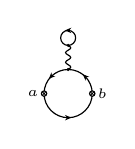
\begin{tikzpicture}[x=0.340cm, y=0.340cm, line width=0.420pt, baseline={([yshift=-0.6ex]0,0)}]
  \draw (0.000,0.900) arc[start angle=90.000, end angle=180.000, radius=0.900];
  \fill (-0.721,0.552) -- (-0.480,0.649) -- (-0.607,0.666) -- (-0.624,0.793) -- cycle;
  \draw (-0.900,0.000) arc[start angle=180.000, end angle=360.000, radius=0.900];
  \fill (0.119,-0.900) -- (-0.119,-0.798) -- (-0.042,-0.900) -- (-0.119,-1.002) -- cycle;
  \draw (0.900,0.000) arc[start angle=0.000, end angle=90.000, radius=0.900];
  \fill (0.552,0.721) -- (0.649,0.480) -- (0.666,0.607) -- (0.793,0.624) -- cycle;
  \draw plot[smooth, tension=0.7] coordinates {(0.000,1.800) (0.069,1.755) (0.097,1.710) (0.069,1.665) (0.000,1.620) (-0.069,1.575) (-0.097,1.530) (-0.069,1.485) (0.000,1.440) (0.069,1.395) (0.097,1.350) (0.069,1.305) (0.000,1.260) (-0.069,1.215) (-0.097,1.170) (-0.069,1.125) (0.000,1.080) (0.069,1.035) (0.097,0.990) (0.069,0.945) (0.000,0.900)};
  \draw (0.000,1.800) arc[start angle=270.000, end angle=630.000, radius=0.280];
  \fill (-0.119,2.360) -- (0.119,2.258) -- (0.042,2.360) -- (0.119,2.462) -- cycle;
  \draw[fill=white] (-0.900,0.000) circle (0.100);
  \draw[line width=0.298pt] (-0.830,0.070) -- (-0.970,-0.070) (-0.830,-0.070) -- (-0.970,0.070);
  \draw[fill=white] (0.900,0.000) circle (0.100);
  \draw[line width=0.298pt] (0.970,0.070) -- (0.830,-0.070) (0.970,-0.070) -- (0.830,0.070);
  \fill (0.000,1.800) circle (0.064);
  \fill (0.000,0.900) circle (0.064);
  \node[font=\tiny, inner sep=0pt, anchor=0] at (-1.090,-0.001) {$a$};
  \node[font=\tiny, inner sep=0pt, anchor=180] at (1.090,-0.001) {$b$};
\end{tikzpicture}}
\diagramgap
\mbox{$\displaystyle -\,$\,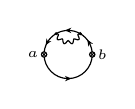
\begin{tikzpicture}[x=0.340cm, y=0.340cm, line width=0.420pt, baseline={([yshift=-0.6ex]0,0)}]
  \draw (-0.450,0.779) arc[start angle=120.000, end angle=180.000, radius=0.900];
  \fill (-0.839,0.347) -- (-0.631,0.502) -- (-0.759,0.486) -- (-0.808,0.604) -- cycle;
  \draw (-0.900,0.000) arc[start angle=180.000, end angle=360.000, radius=0.900];
  \fill (0.119,-0.900) -- (-0.119,-0.798) -- (-0.042,-0.900) -- (-0.119,-1.002) -- cycle;
  \draw (0.450,0.779) arc[start angle=60.000, end angle=120.000, radius=0.900];
  \fill (-0.119,0.900) -- (0.119,0.798) -- (0.042,0.900) -- (0.119,1.002) -- cycle;
  \draw plot[smooth, tension=0.7] coordinates {(-0.450,0.779) (-0.394,0.766) (-0.363,0.748) (-0.368,0.713) (-0.393,0.660) (-0.412,0.604) (-0.404,0.562) (-0.363,0.549) (-0.305,0.562) (-0.250,0.580) (-0.215,0.581) (-0.200,0.549) (-0.193,0.491) (-0.179,0.433) (-0.150,0.402) (-0.109,0.413) (-0.066,0.455) (-0.030,0.500) (0.000,0.519) (0.030,0.500) (0.066,0.455) (0.109,0.413) (0.150,0.402) (0.179,0.433) (0.193,0.491) (0.200,0.549) (0.215,0.581) (0.250,0.580) (0.305,0.562) (0.363,0.549) (0.404,0.562) (0.412,0.604) (0.393,0.660) (0.368,0.713) (0.363,0.748) (0.394,0.766) (0.450,0.779)};
  \draw (0.900,0.000) arc[start angle=360.000, end angle=420.000, radius=0.900];
  \fill (0.720,0.553) -- (0.751,0.296) -- (0.800,0.414) -- (0.927,0.398) -- cycle;
  \draw[fill=white] (-0.900,0.000) circle (0.100);
  \draw[line width=0.298pt] (-0.830,0.070) -- (-0.970,-0.070) (-0.830,-0.070) -- (-0.970,0.070);
  \draw[fill=white] (0.900,0.000) circle (0.100);
  \draw[line width=0.298pt] (0.970,0.070) -- (0.830,-0.070) (0.970,-0.070) -- (0.830,0.070);
  \fill (-0.450,0.779) circle (0.064);
  \fill (0.450,0.779) circle (0.064);
  \node[font=\tiny, inner sep=0pt, anchor=1] at (-1.090,-0.002) {$a$};
  \node[font=\tiny, inner sep=0pt, anchor=179] at (1.090,-0.002) {$b$};
\end{tikzpicture}}
